\documentclass[final,a4paper,twocolumn,11pt]{report}
\usepackage{graphicx}
\usepackage[T1]{fontenc}
\usepackage[utf8]{inputenc}
\usepackage{amsmath}
\usepackage{comment}
\usepackage{amssymb}
\usepackage{polski}
\usepackage[polish]{babel}
\usepackage{float}
\usepackage{enumitem}
\usepackage{indentfirst}
\usepackage{caption}
\usepackage{subcaption}
\usepackage{yfonts}
\usepackage{braket}
\usepackage[margin=2cm]{geometry}
\usepackage{tabularx}
\usepackage{booktabs}
\usepackage{hyperref}
\hypersetup{
    colorlinks=true,
    linkcolor=black,
    urlcolor=red
}
\usepackage[nospace,polish]{varioref}
\usepackage{siunitx}
\DeclareSIUnit\litre{l}
\DeclareSIUnit{\arbitrary}{a.u.}
\sisetup{
    per-mode=symbol,
    exponent-product=\times,
    range-units=repeat,
    range-open-phrase={od },
    output-decimal-marker={.},
    product-units=repeat
}

%\usepackage[version=4]{mhchem}
    
% \usepackage{tikz}
% \usetikzlibrary{positioning, arrows.meta, calc}

% \usepackage{listings}
% \lstset{
%   basicstyle=\ttfamily\small,
%   breaklines=false,
%   frame=single
% }

\captionsetup[figure]{name=Wykres}

\title{\Huge{\textgoth{Quantum Point Contact}}}
\author{\Huge{\textfrak{Maciej Flaga}}}
\date{}

\begin{document}
\maketitle

\chapter{Realizacja}

\section{Relacja dyspersji}

Zaczęto od wyznaczenia relacji dyspersji dla układu jednorodnego ($V=0$). 
W tym celu założono symetrię translacyjną wzdłuż $x$ i skupiono się na pojedynczym przekroju (komórce elementarnej).

Rozwiązano problem własny oznaczony numerem (5) w treści zadania wielokrotnie dla różnych wartości $k_x$ z pierwszej strefy Brillouina -- każdorazowo otrzymując $N_y$ wartości własnych.  
W tym celu posłużono się biblioteką \texttt{GSL} i jej funkcją \texttt{gsl\_eigen\_symm} ze względu na rzeczywistą, symetryczną postać hamiltonianu.

Wykreślono poszczególne poziomy energetyczne w funkcji pędu (Wykres \ref{dyspfile}).

\begin{figure}[h]
    \centering
    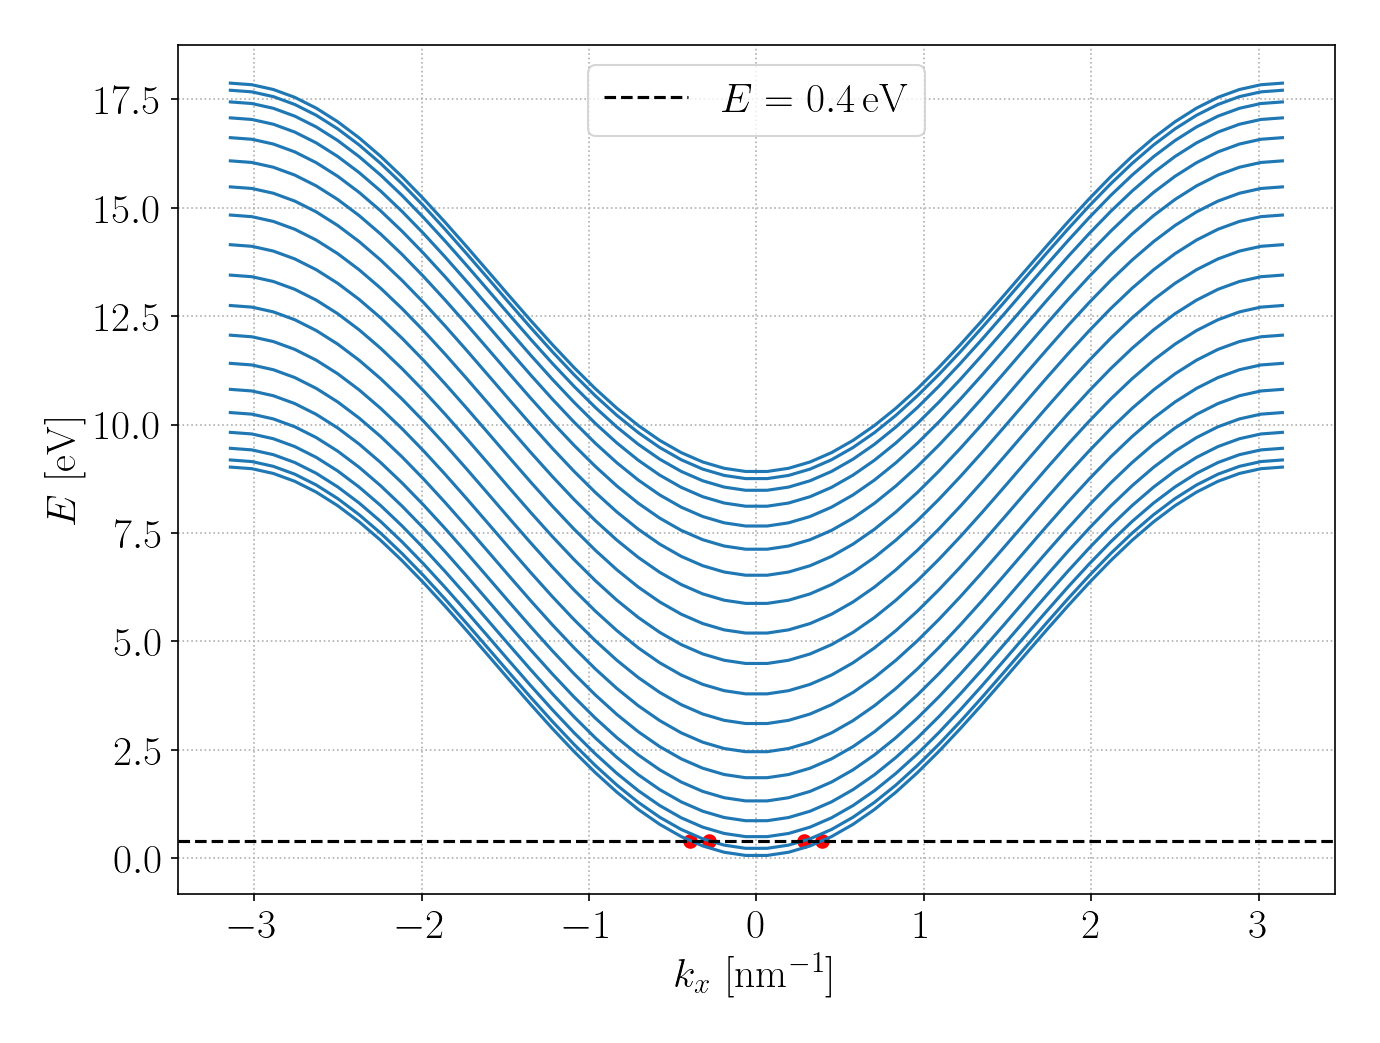
\includegraphics[width=\linewidth]{figures/dyspfile04.png}
    \caption{Relacja dyspersji}
    \label{dyspfile}
\end{figure}

\section{Mody poprzeczne}

Kolejnym krokiem było wyznaczenie modów poprzecznych poprzez rozwiązanie uogólnionego problemu własnego. 

Ze względu na to, że \texttt{GSL} nie obsługuje zespolonych macierzy niehermitowskich zdecydowano posłużyć się biblioteką \texttt{Eigen}. 
Zaprogramowano funkcję \texttt{upw\_inv}.
Funkcja rozwiązuje problem poprzez najpierw odwrócenie macierzy diagonalnej B i sprowadzenie uogólnionego problemu własnego do zwykłego problemu własnego a następnie korzysta z gotowej funkcji \texttt{ComplexEigenSolver}.

Rozwiązaniem takiego problemu jest $2N_y$ wartości i wektorów własnych.
Ze względu na to jak zdefiniowany był nasz problem interesuje nas jedynie połowa wartości i wektorów (skróconych o połowę)\footnote{Ze względu na próby debugowania, kod zwraca $2N_y$ wartości i wektorów własnych (wciąż skróconych o połowę) a następnie nakładany jest warunek $|\lambda|=1 \wedge  \Im(\lambda)<0$ do wyznaczenia $\lambda_{-,n}$}.
Otrzymane funkcje własne $\mathbf{u}_n$ znormalizowano do 1.

Widzimy, że uzyskano mody poprzeczne i zanikające. 
Dla modów poprzecznych wyznaczono wartości $k_x^{-,n}$ (czerwone punkty na Wykresie \ref{dyspfile}) i $v_{-,n}$ oraz wykreślono funkcje falowe (Wykres \ref{popU}).

\begin{figure}[h]
    \centering
    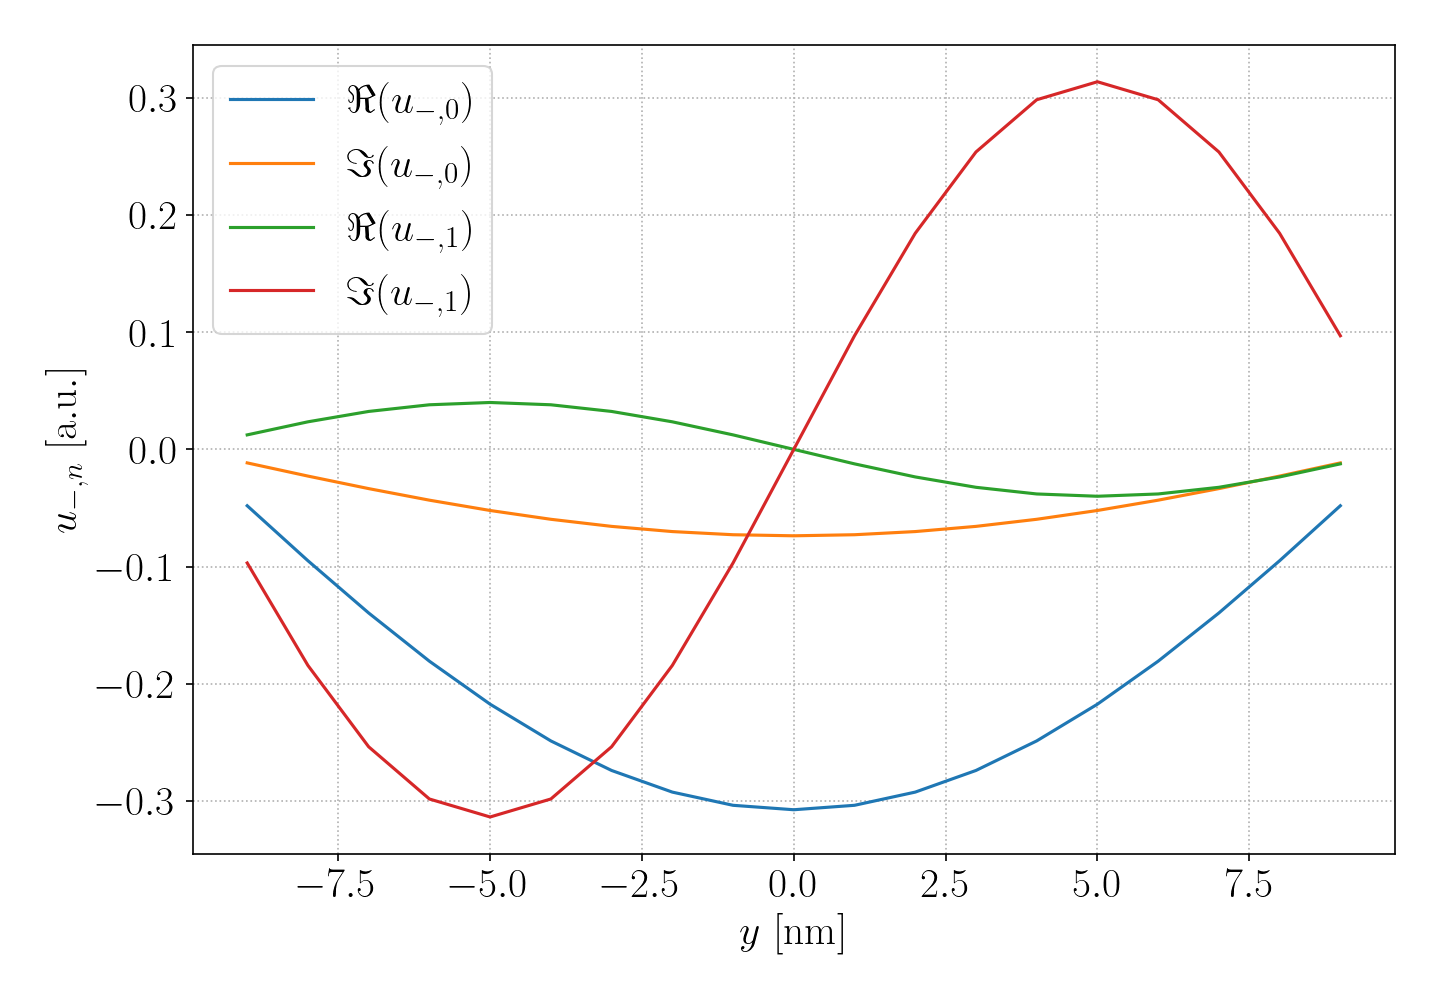
\includegraphics[width=\linewidth]{figures/popU04.png}
    \caption{Znormalizowane mody poprzeczne}
    \label{popU}
\end{figure}

Wykresy dla $E=\qty{0.2}{\electronvolt}$ wraz z pełnym rozwiązaniem układu przedstawione są na końcu sprawozdania.

\section{Współczynnik Transmisji}

\subsection{Układ}

Zdefiniowano układ jako kanał o wymiarach \qtyproduct{1x0.7}{\micro\meter} z potencjałem emulującym bramkę po środku.
Mapa potencjału przedstawiona jest na Wykresie \ref{potfile}.

\begin{figure}[h]
    \centering
    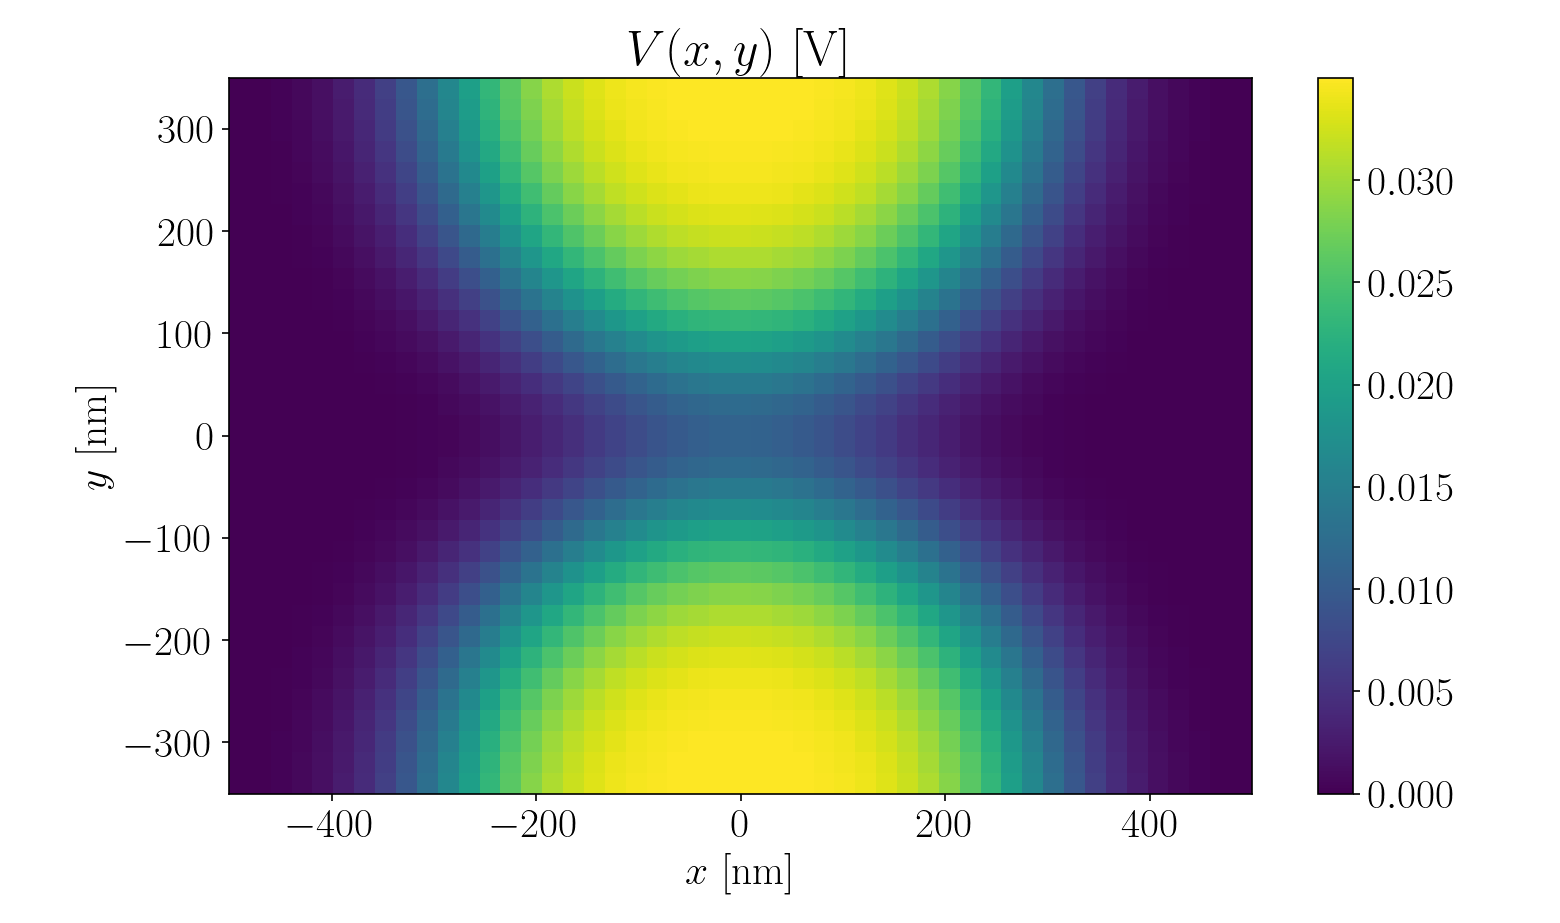
\includegraphics[width=\linewidth]{figures/potfile.png}
    \caption{Potencjał QPC}
    \label{potfile}
\end{figure}

\subsection{Omówienie kodu}

\subsubsection{Znalezienie $\psi$}

Napisano funkcję \texttt{znajdzPsi}, która definiuje i rozwiązuje układ równań oznaczony jako (11) w treści zadania dla ustalonego potencjału oraz $c_{in}$. 
Układ macierzowy jest rozwiązywany metodą rozkładu LU przy pomocy biblioteki \texttt{Eigen}. 

Taki układ rozwiązano dla każdego modu poprzecznego otrzymując $n$ funkcji falowych.

\subsubsection{Obliczenie T i R}

Dla każdego $n$-tego modu przeprowadzono obliczenia współczynników $c_{out,m}$ oraz $d_{out,m}$, które następnie porównano z współczynnikiem $c_{in,n}$ uzyskując prawdopodobieństwo transmisji $(T_n)$ oraz odbicia $(R_n)$ danego modu.
Zsumowano współczynniki po modach otrzymując całkowite prawdopodobieństwo transmisji/odbicia.

Wyniki są wypisywane do terminala przy uruchomieniu kodu.

\subsection{Wyniki}

Przeprowadzono obliczenia\footnote{Z uwagi na konieczność restrukturyzacji kodu zdecydowano się pracować na innej gałęzi gitowskiej i ta część kodu nie jest uwzględniona w plikach C++.} współczynników $T$ i $R$ dla $E=\qty{0.015}{\electronvolt}$ z potencjałem bramek $V_{gates}$ w zakresie \qtyrange{-1.3}{-0.7}{\volt} z krokiem \qty{0.02}{\volt}. 

Wyniki przedstawione są na Wykresach \ref{Tfile}, \ref{Rfile} i \ref{TRfile}.

\begin{figure}[h]
    \centering
    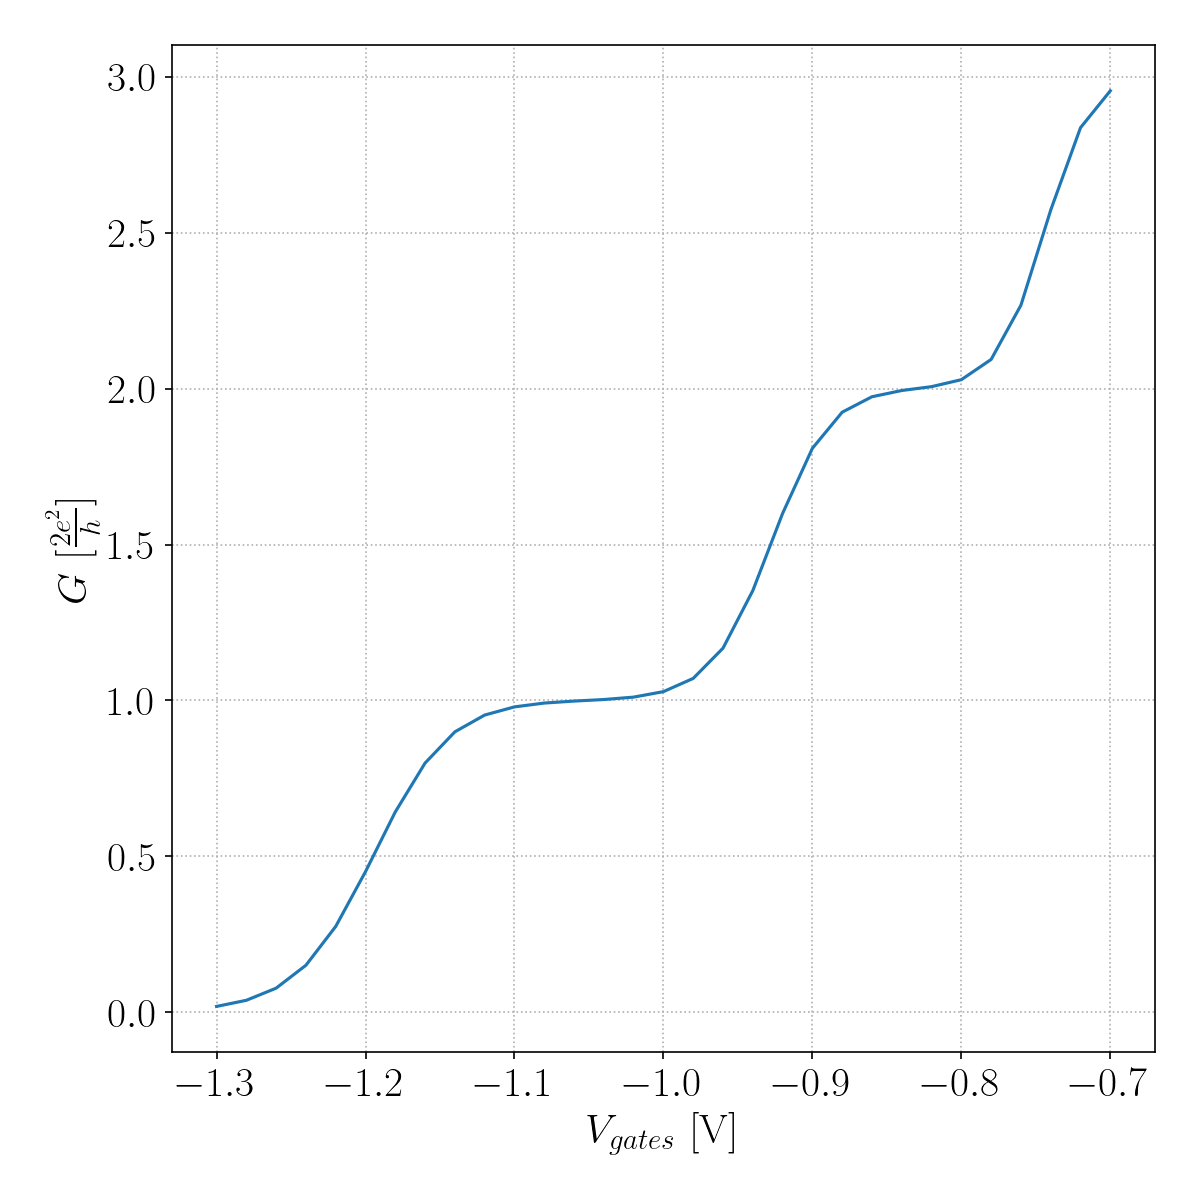
\includegraphics[width=\linewidth]{figures/Tfile.png}
    \caption{Konduktancja w funkcji potencjału bramek}
    \label{Tfile}
\end{figure}

\begin{figure}[h]
    \centering
    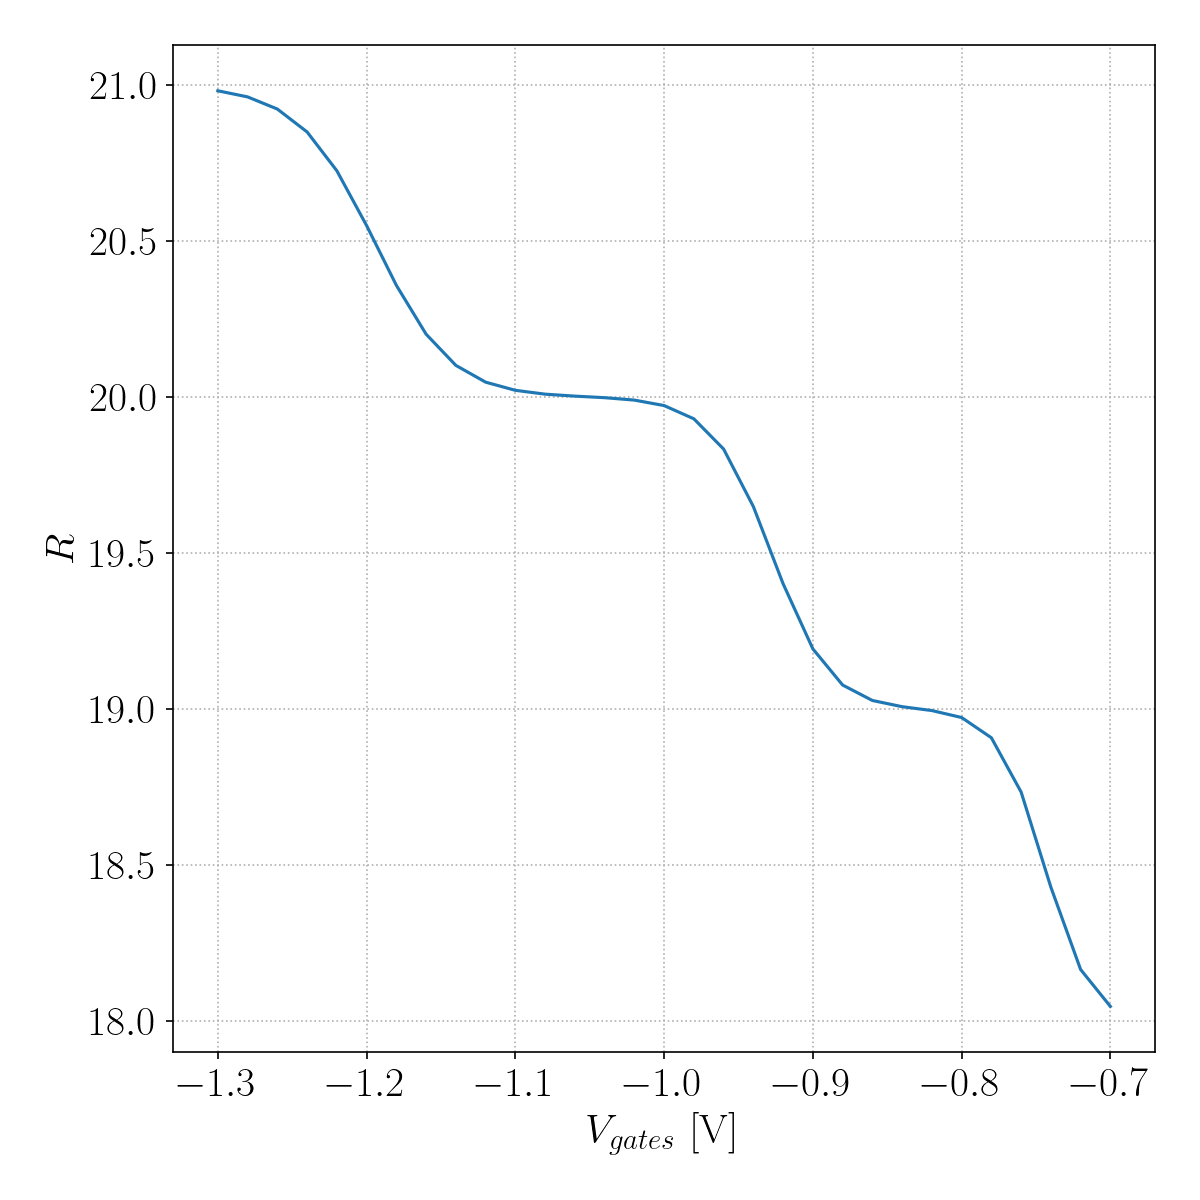
\includegraphics[width=\linewidth]{figures/Rfile.png}
    \caption{Współczynnik odbicia w funkcji potencjału bramek}
    \label{Rfile}
\end{figure}

\begin{figure}[h]
    \centering
    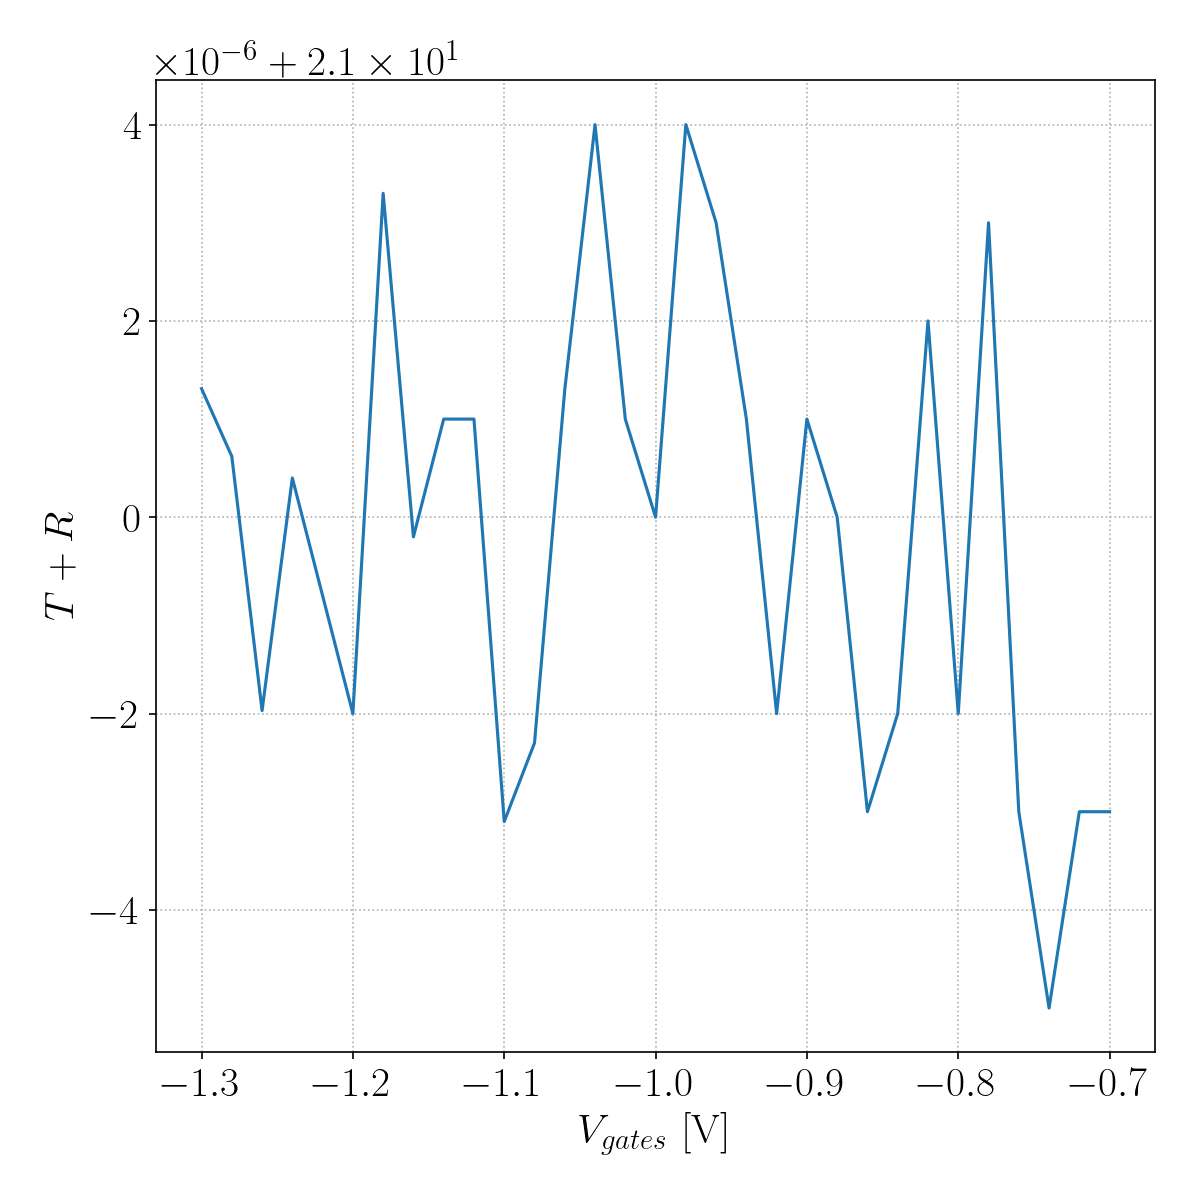
\includegraphics[width=\linewidth]{figures/TRfile.png}
    \caption{Suma współczynników transmisji i odbicia (równa liczbie modów poprzecznych)}
    \label{TRfile}
\end{figure}
\newpage
\section{Gęstość elektronów}

Obliczono gęstość elektronową ze wzoru

\begin{align*}
    \rho(x,y)=|\Psi(x,y)|^2=\sum_{n}|\psi_n(x,y)|^2,
\end{align*}

\noindent gdzie $n$ oznacza $n$-ty mod poprzeczny, dla potencjału $V_{gates}$ odpowiadającemu $G=0$, $G=G_0$ oraz $G=2G_0$.

Wyniki przedstawiają Wykresy \ref{rhofile0G}, \ref{rhofile1G} oraz \ref{rhofile2G}.
Widzimy jak otwierają się kolejne kanały przepływu.

Warto zaznaczyć, że funkcja $\rho(x,y)$ najprawdopodobniej nie jest znormalizowana.

\begin{figure}[h]
    \centering
    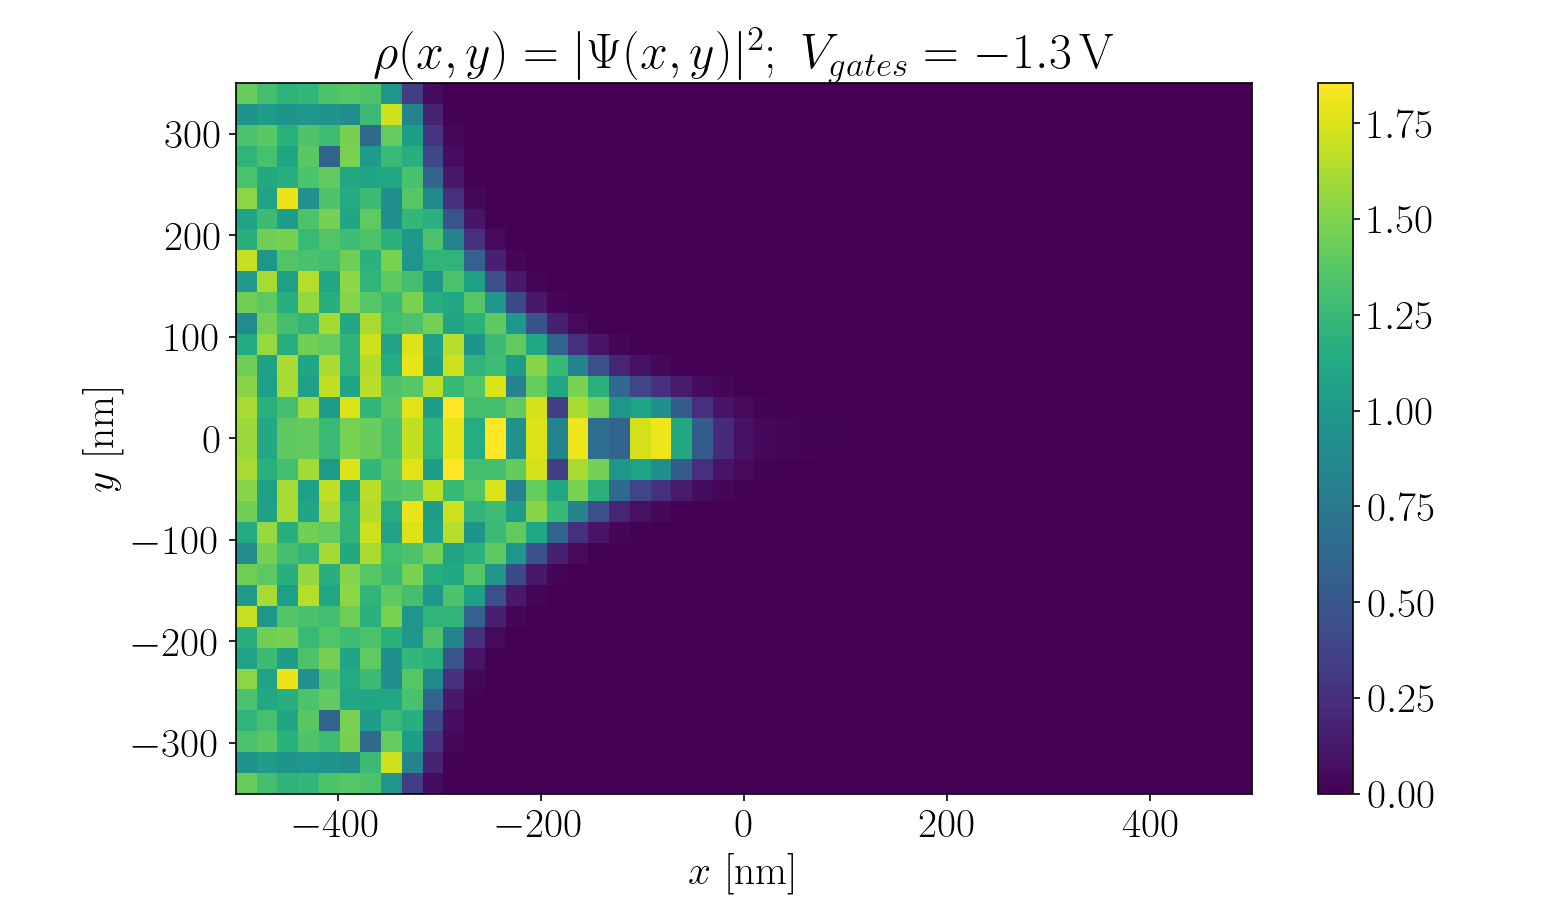
\includegraphics[width=\linewidth]{figures/rhofile0G.png}
    \caption{Gęstość elektronowa dla $G=0$}
    \label{rhofile0G}
\end{figure}

\begin{figure}[h]
    \centering
    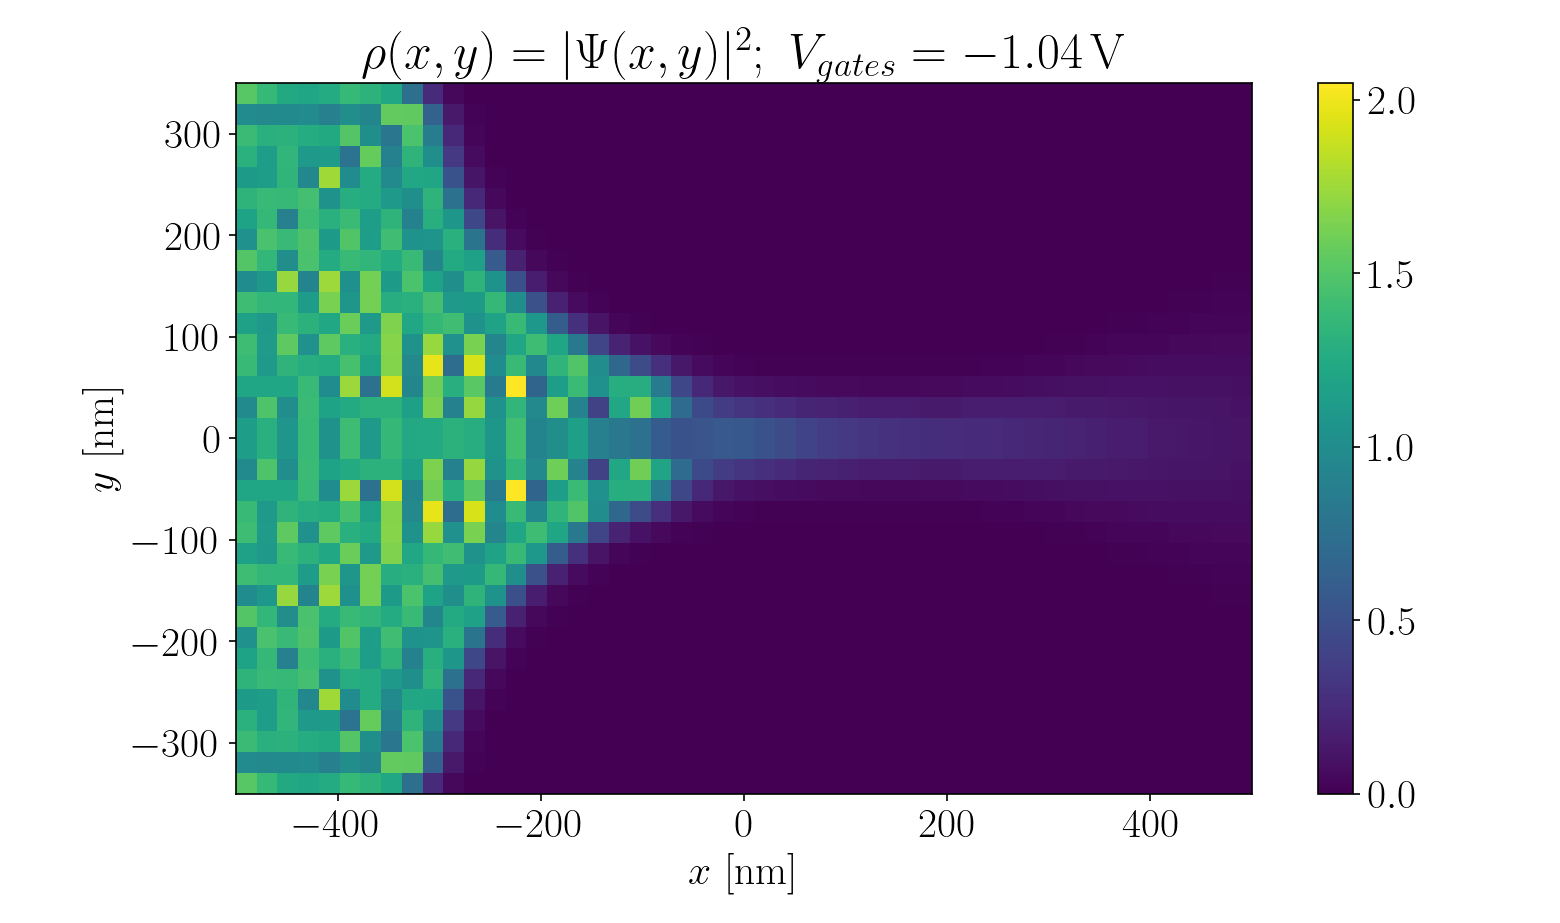
\includegraphics[width=\linewidth]{figures/rhofile1G.png}
    \caption{Gęstość elektronowa dla $G=G_0$}
    \label{rhofile1G}
\end{figure}

\begin{figure}[h]
    \centering
    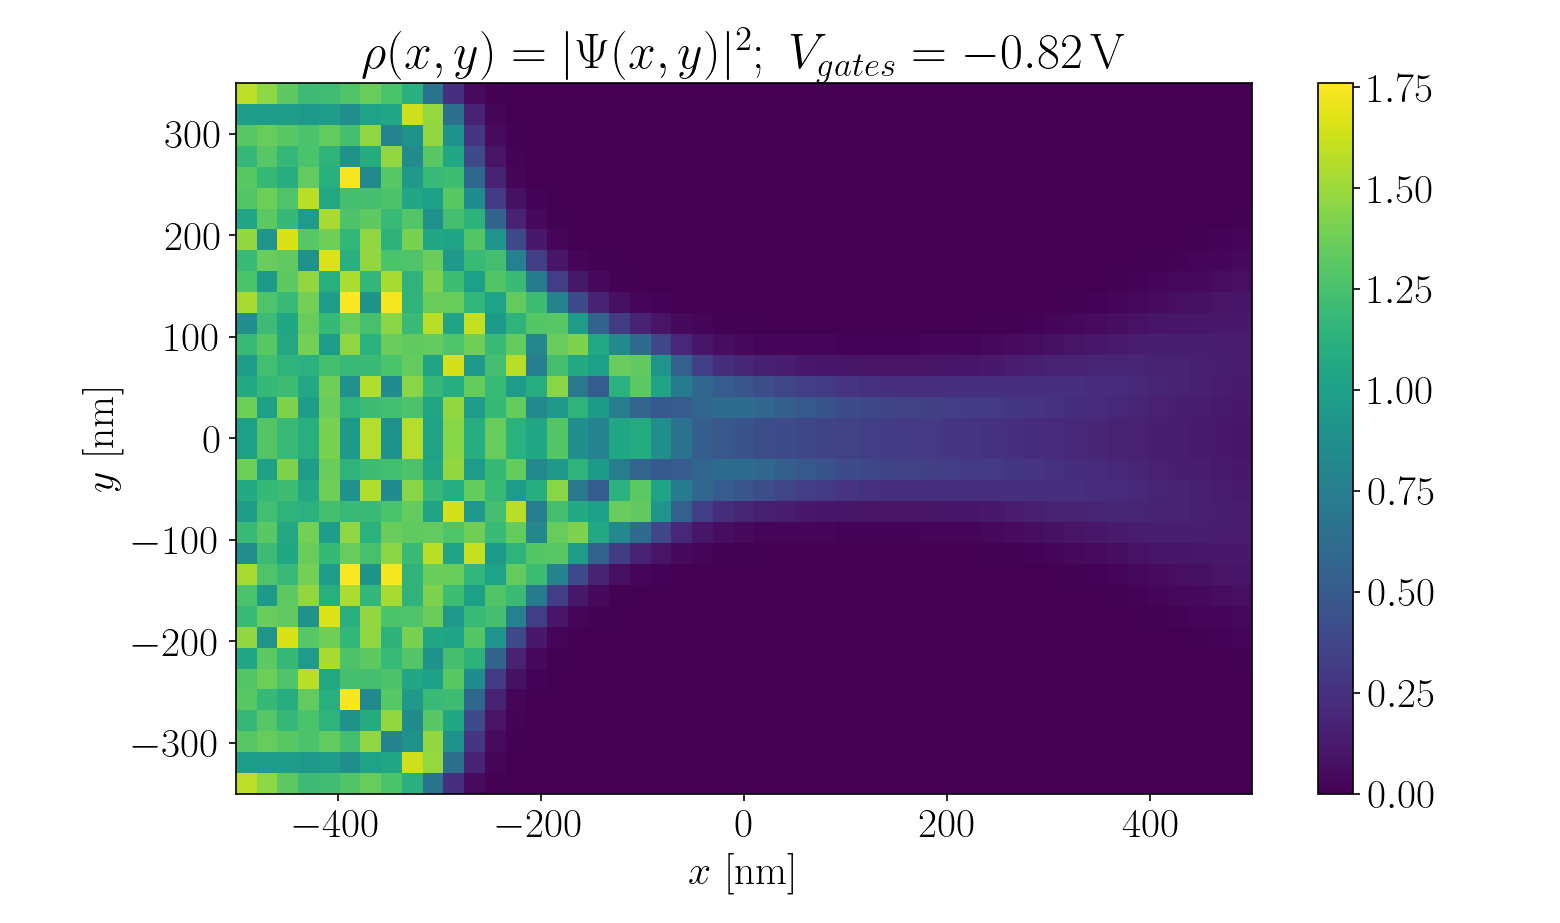
\includegraphics[width=\linewidth]{figures/rhofile2G.png}
    \caption{Gęstość elektronowa dla $G=2G_0$}
    \label{rhofile2G}
\end{figure}

\section{Animacja}

Z racji, że program i tak liczył wszystkie funkcje falowe do wyznaczenia współczynników $T$ i $R$ przy zadanym potencjale, zdecydowano się zapisać również funkcję gęstości elektronowej w każdym kroku. 
Sporządzono animację (\texttt{figures/anim.mp4}), która przedstawia jak zmienia się gęstość przy ciągłej zmianie potencjału.

Tym razem potencjał zmieniał się w zakresie \qtyrange{-1.3}{-0.5}{\volt}, przy czym dla niższego (co do wartości bezwzględnej) potencjału wyniki mogą być niefizyczne ponieważ cząstka ma za dużą energię w porównaniu z układem. Należałoby zwiększyć wartość $N_y$ aby udoskonalić wyniki.
Mogę się jednak mylić.

\onecolumn

\section{Reszta wykresów}

\begin{figure}[h]
    \centering
    \begin{subfigure}[t]{0.49\linewidth}
        \centering
        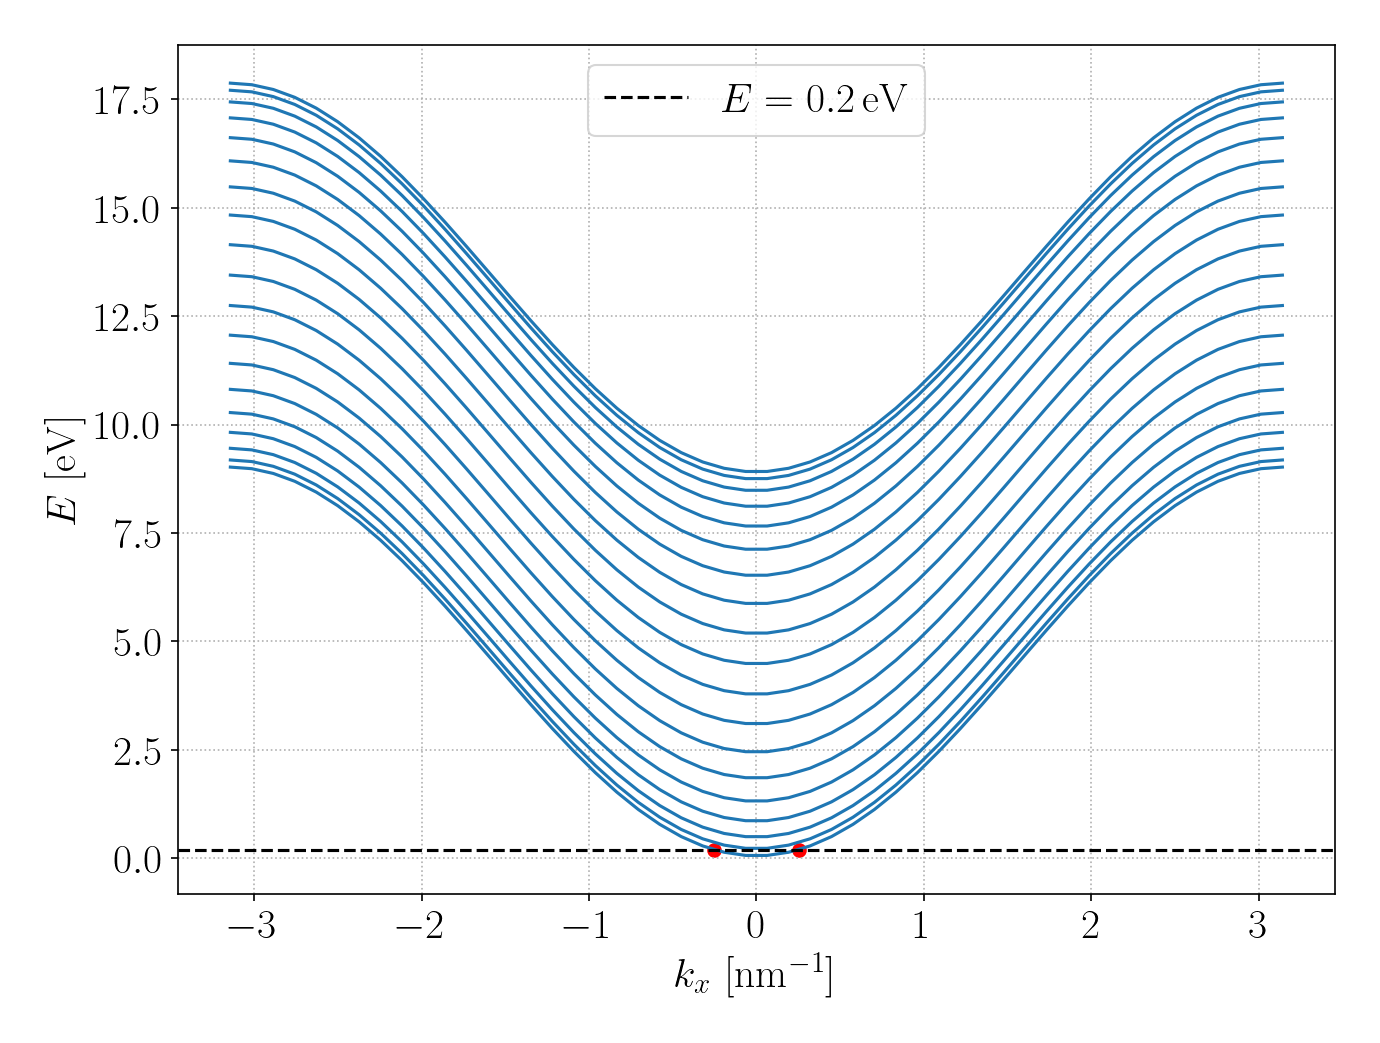
\includegraphics[width=\linewidth]{figures/dyspfile02.png}
        \caption{Relacja dyspersji}
        \label{dyspfile02}
    \end{subfigure}
    \hfill
    \begin{subfigure}[t]{0.49\linewidth}
        \centering
        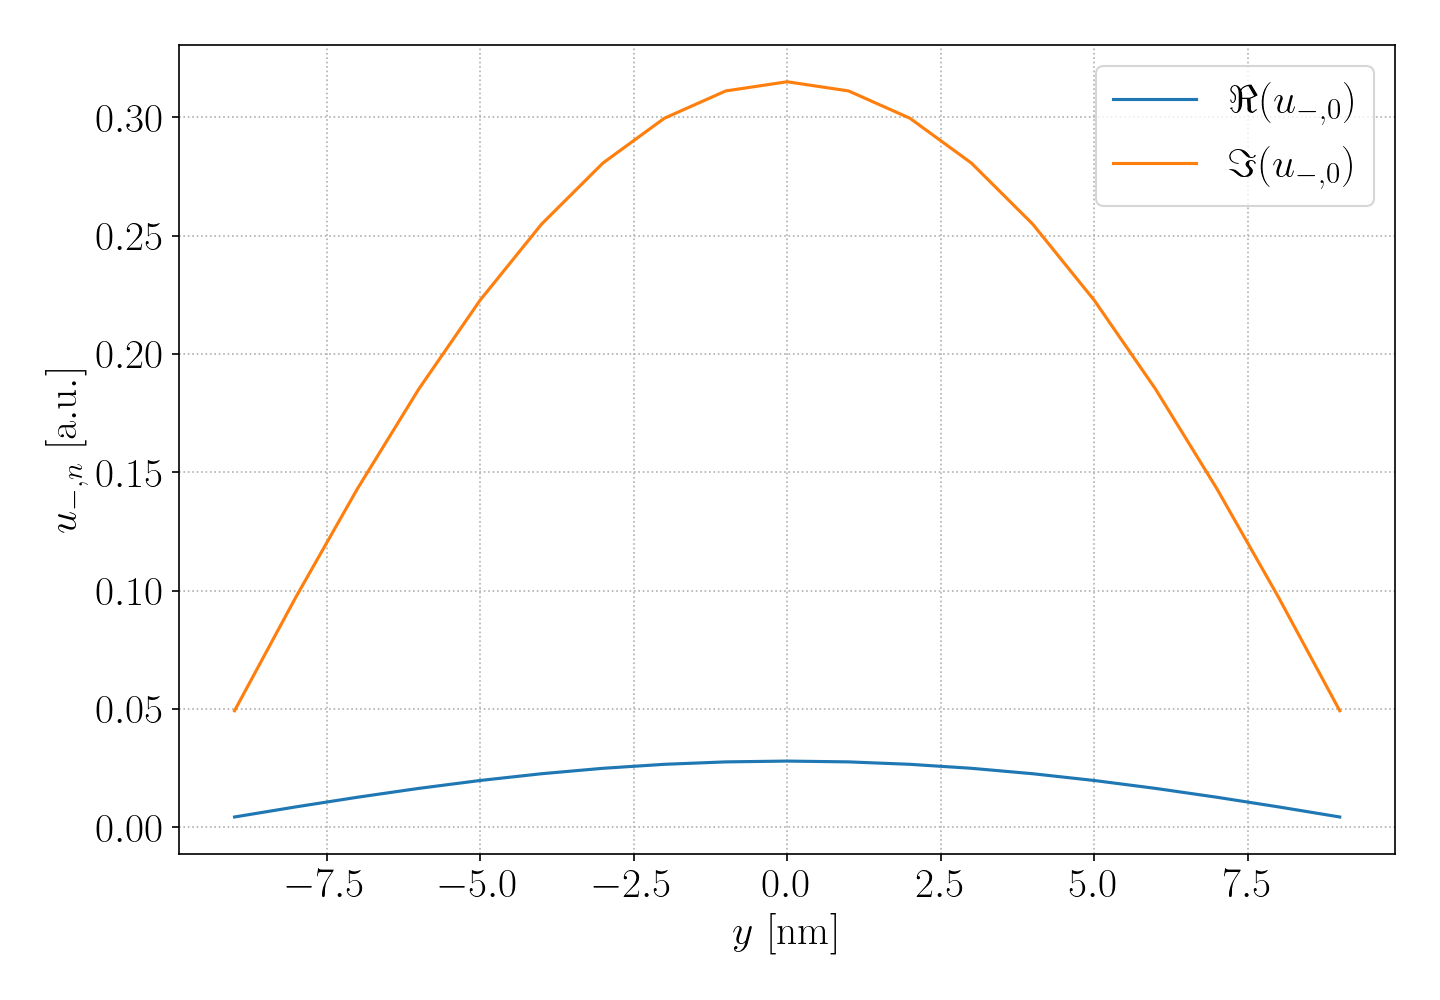
\includegraphics[width=\linewidth]{figures/popU02.png}
        \caption{Mody poprzeczne}
        \label{popU02}
    \end{subfigure}
    \caption{Wyniki dla $E=\qty{0.2}{\electronvolt}$}
    \label{02}
\end{figure}

\begin{figure}[h]
    \centering
    \begin{subfigure}[t]{0.5\linewidth}
        \centering
        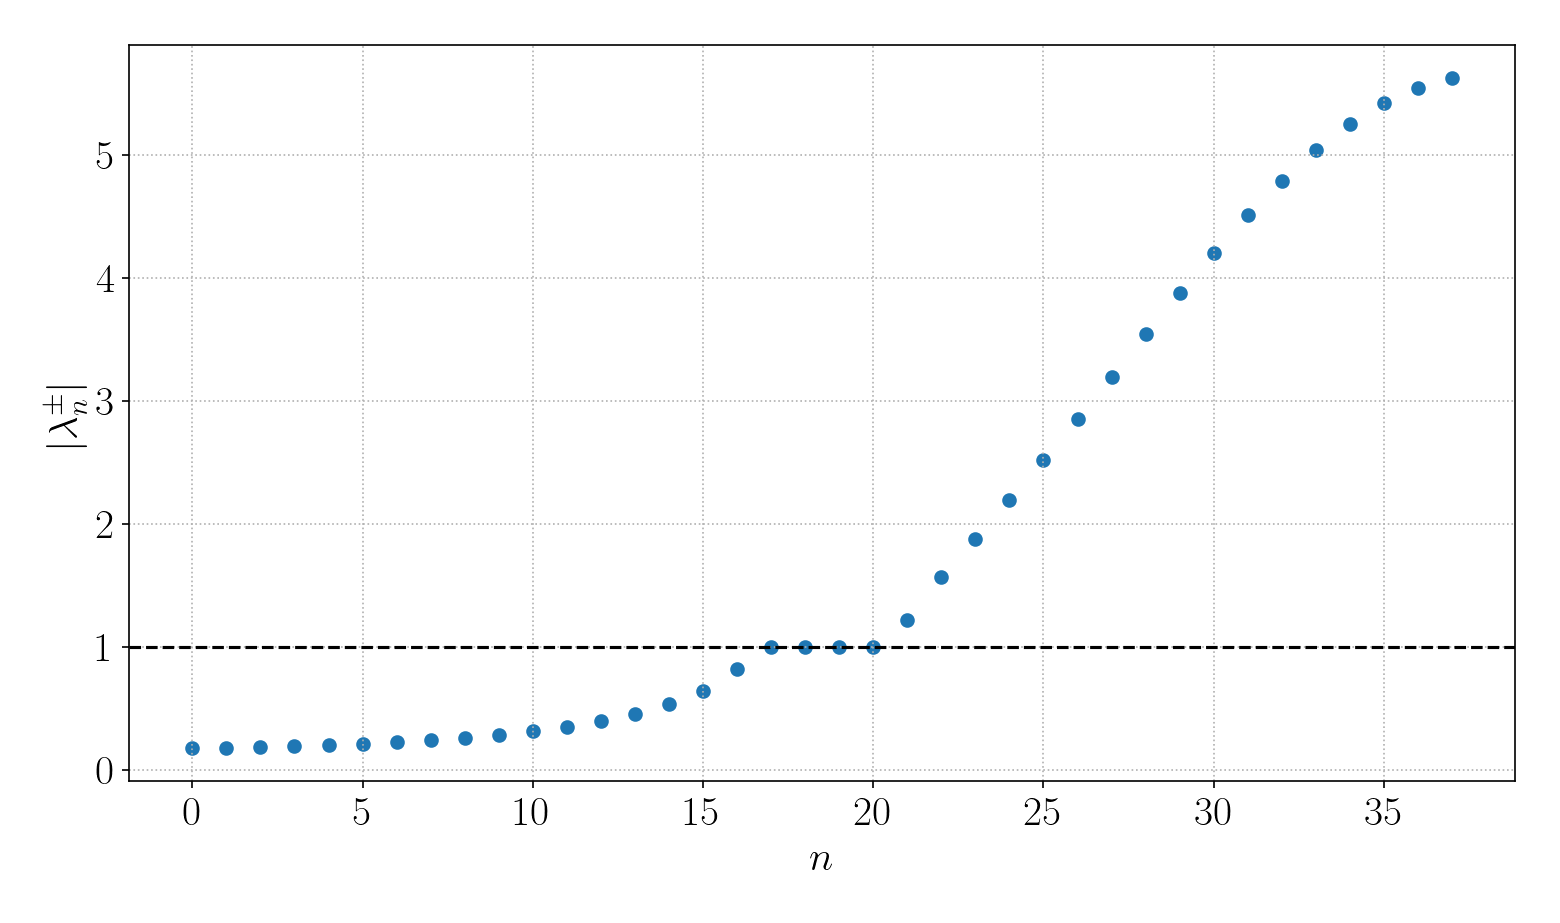
\includegraphics[width=\linewidth]{figures/lfile.png}
        \caption{Wartości własne}
        \label{lfile}
    \end{subfigure}
    \vfill
    \begin{subfigure}[t]{0.49\linewidth}
        \centering
        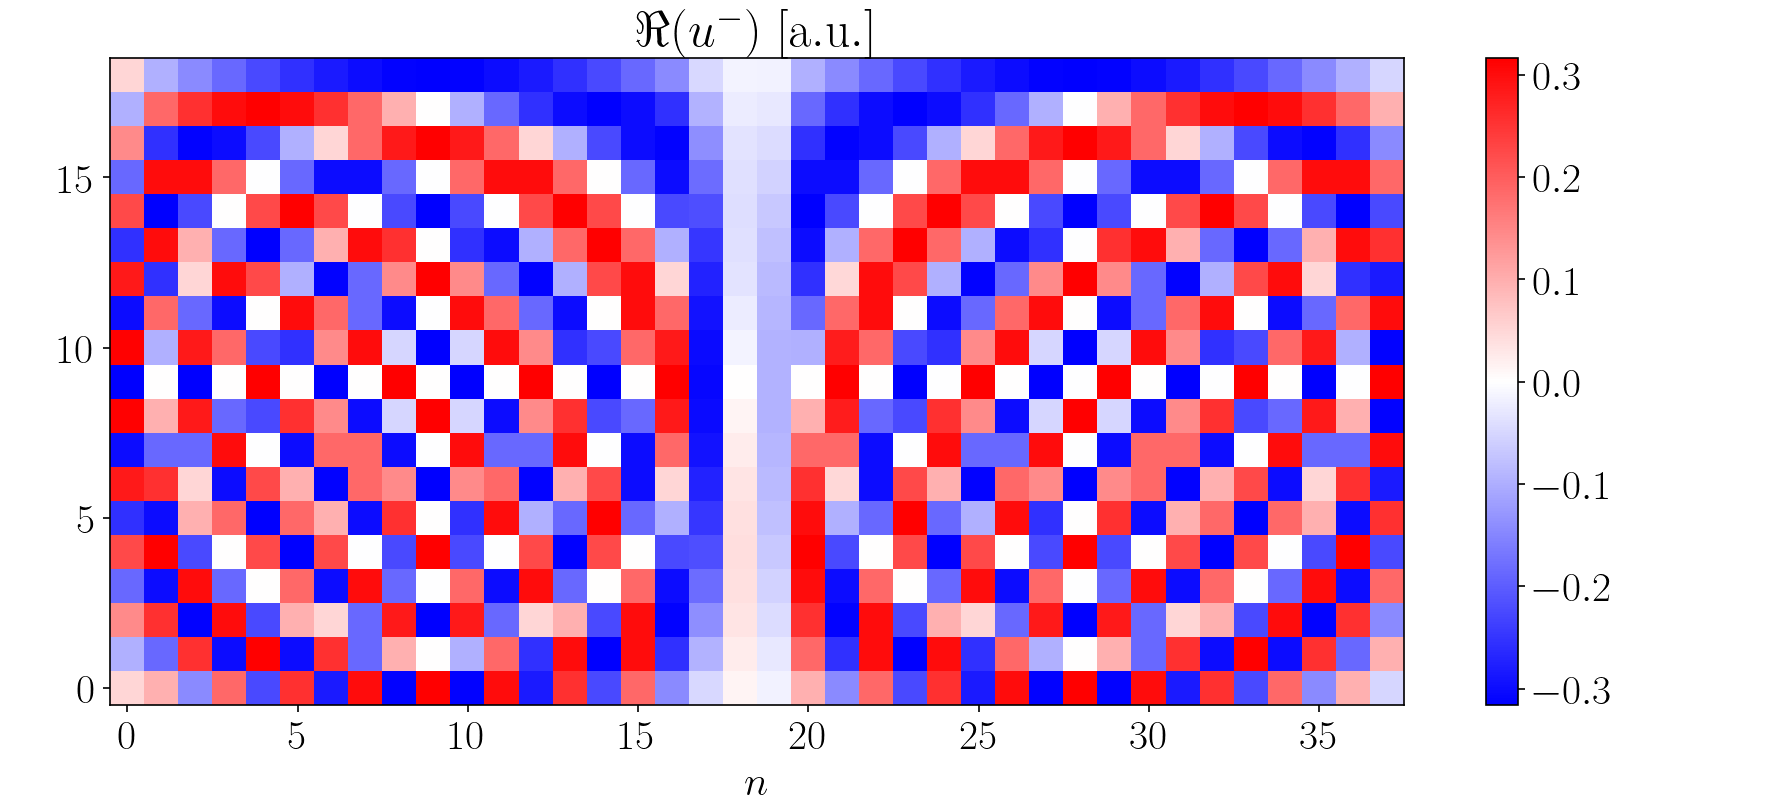
\includegraphics[width=\linewidth]{figures/uRe.png}
        \caption{Część rzeczywista wektorów własnych}
        \label{uRe}
    \end{subfigure}
    \hfill
    \begin{subfigure}[t]{0.49\linewidth}
        \centering
        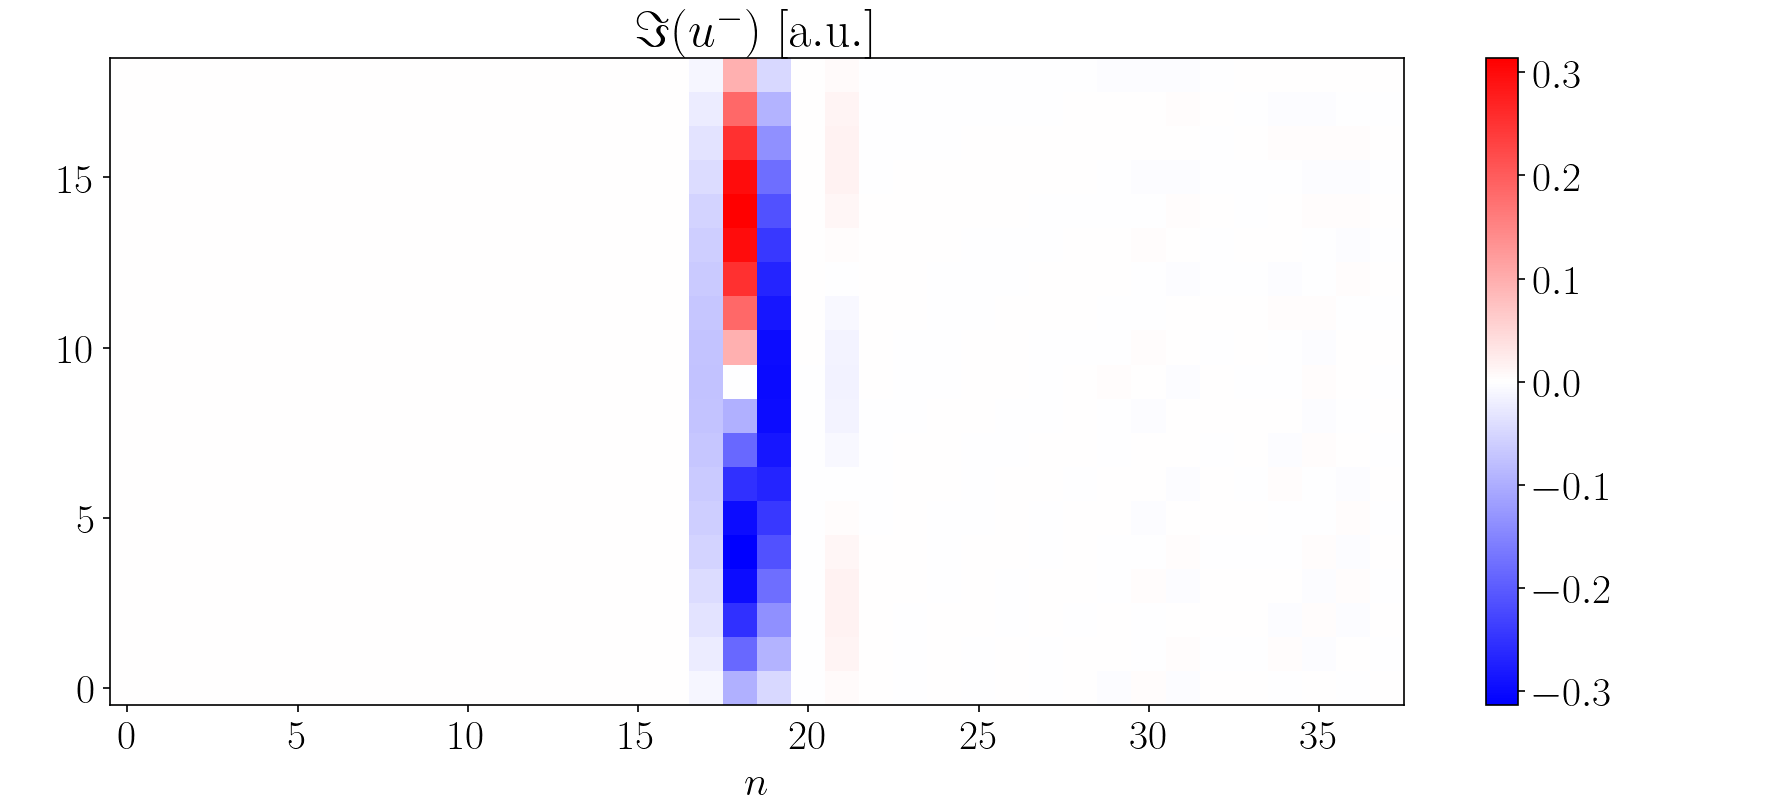
\includegraphics[width=\linewidth]{figures/uIm.png}
        \caption{Część urojona wektorów własnych}
        \label{uIm}
    \end{subfigure}
    \caption{Rozwiązanie układu z sekcji $\mathbf{1.2}$}
    \label{12}
\end{figure}

\end{document}
